\section{系统开发与实现}

\subsection{结构化开发方式}

结构化方法是一种传统的软件开发方法,它是由结构化分析、结构化设计和结构化程序设计三部分有机组合而成的。结构化设计方法是以自顶向下,逐步求精,模块化为基点,以模块化,抽象,逐层分解求精,信息隐蔽化局部化和保持模块独立为准则的设计软件的数据架构和模块架构的方法学。它的要点是是把一个复杂问题的求解过程分阶段进行,而且这种分解是自顶向下,逐层分解,使得每个阶段处理的问题都控制在容易理解和处理的范围内。

结构化方法的基本思想主要体现在三个方面。

(1)自顶向下,逐步求精:把程序看成是一个逐步演化的过程。把一个系统与程序看成是一层一层的。本次的系统开发中,按照自顶向下方式。基于Arduino的分布式温度控制系统可分为:数据收集,数据传输,数据展示,用户管理等几个子系统,而每个子系统又划分为接收/发送信息,实施处理,提供返回信息等等部分。

(2)模块化:即将几个系统分成几个模块,每个模块实现特定的功能,最终整个系统由这些模块组成。模块跟模块之间通过接口传递信息,模块最重要的特点就是独立性,模块之间还有上下层的关系,上层模块调用下层模块来实现一些功能。本系统的模块化图如下图\ref{fig:4-1}所示

\begin{figure}[htbp]
	\centering
	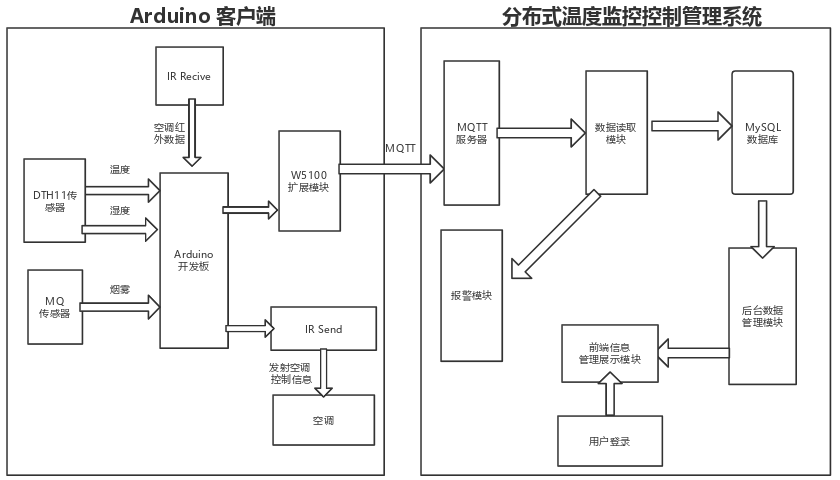
\includegraphics[width=\linewidth]{figure/4-1}
	\caption{温度控制系统模块图}
	\label{fig:4-1}
\end{figure}

(3)语句结构化:顺序结构、分支结构、循环结构,都是常用的语句结构。

结构化分析方法的实质是着眼于数据流,自顶向下,逐层分解,建立系统的处理流程,以数据流图和数据字典为主要工具,建立系统的逻辑模型。

结构化分析的步骤如下:

(1)通过对计划任务书的需求分析为背景,确立整个系统的具体模型

(2)去掉具体模型中非本质因素,抽象出当前系统的逻辑模型

(3)根据计算机的特点分析当前系统与目标系统的差别,建立目标系统的逻辑模型

(4)完善目标系统并补充细节,写出目标系统的软件需求规格说明

(5)测试直到确认满足计划任务书对软件的需求

结构化设计方法给出一组帮助设计人员在模块层次上区分设计质量的原理与技术。它通常与结构化分析方法衔接起来使用,以数据流图为基础得到软件的模块结构。SD方法尤其适用于变换型结构和事务型结构的目标系统。在设计过程中,它从整个程序的结构出发,利用模块结构图表述程序模块之间的关系。


% \subsection{基于 Git 的版本控制和多人协作}

% Git 是一个版本控制系统,用于跟踪计算机文件的变化,并在多个人员之间协调对这些文件的工作。它主要用于软件开发中的源代码版本控制,同时它也可以用来跟踪我们的任何一个文件的变化过程。作为一个分布式的版本控制系统,它的主要特性是高速、数据完整性和对分布式、非线性工作流的支持。

% Git 是由 Linus Torvalds 在 2005 年创建的,当时用于开发 Linux 内核,其他内核开发人员也为其最初的开发做出了贡献。Junio Hamano则是目前的维护者。Git 不同与大多数客户机 — 服务器系统(C/S System),每个计算机上的每个 Git 目录都是一个完整的存储库,具有完整的历史和完整的版本跟踪功能,独立于网络访问或中央服务器。

% 如图 \ref{git-flow} 所示,Git 的最大优点之一是它的分支功能。与其他集中式的版本控制系统的不同点在于,Git 分支是廉价且易于合并的。这使得特性分支工作流受到许多 Git 用户的欢迎。
% 特性分支为代码库的每个更改提供一个隔离的环境。当一个开发人员想要开始做一些事情 —— 不管他们有多大或多么小的时候 —— 他们会创建一个新的分支。这确保了主分支总是包含生产质量代码。

% \begin{figure}
% 	\centering
% 	\includegraphics[width=0.6\linewidth]{figure/git-flow}
% 	\caption{基于 Git 的工作流}
% 	\label{git-flow}
% \end{figure}

% 使用特性分支不仅比直接编辑生产代码更可靠,而且还提供了有组织的开发。例如,在之后针对本系统的完善时可以新建feature分支,代成熟后在和入主分支。确保了主分支的稳健性。

% 特性分支、分布式开发、Pull Request 和稳定的社区环境的最终结果是一个更快的发布周期。这些功能促进了敏捷的工作流,鼓励开发人员更频繁地共享较小的更改。例如,我们可以配置 Git,以便在任何人将一个 pull 请求合并到测试服务器时,将最新的提交从开发分支部署到测试服务器。将这种构建自动化与单元测试结合,让代码从开发阶段转向生产阶段时,对代码质量拥有最高的信心。

% Git 在用户如何管理更新方面提供了很大的灵活性。当在 Git 中与团队合作开发时,确保团队的开发方向是非常重要的。本系统的代码已在在线代码托管平台提供商码云(Gitee)\footnote{基于Arduino的分布式温度控制系统开源地址:\url{https://gitee.com/xsyu_security/arduino.io}}全部开源。
% 选择码云服务主要原因在于:

% \begin{itemize}
% 	\item 国内的Git服务拥有更快的访问速度
% 	\item 私有库功能对个人开发者免费
% 	\item 线上自动代码质量分析
% 	\item 中文语言便于团队成员上手
% \end{itemize}

% Git非常受欢迎,被广泛使用,并被开发人员社区中绝大多数人接受为标准版本控制系统。在大量的Git用户组成的社区可以让我们寻求外部帮助并轻松解决问题。答辩系统业务的开发严重依赖于软件开发流程,Git将彻底改变了我们团队创建和交付工作的方式。包括设计、开发、产品管理、上线运行、客户支持在内的各种流程都可以在开发团队中使用Git轻松处理和维护。

\subsection{红外编码}
红外通信是利用近红外波段的红外线作为传递信息的媒体,即通信信道。发送端将基带二进制信号调制为一系列的脉冲串信号,通过红外发射管发射红外信号。接收端将接收到的光脉转换成电信号,再经过放大、滤波等处理后送给解调电路进行解调,还原为二进制数字信号后输出。常用的有通过脉冲宽度来实现信号调制的脉宽调制(PWM)和通过脉冲串之间的时间间隔来实现信号调制的脉时调制(PPM)两种方法。 简而言之,红外通信的实质就是对二进制数字信号进行调制与解调,以便利用红外信道进行传输;红外通信接口就是针对红外信道的调制解调器。二进制数字信号如何进行调制与解调,利用何种红外信道进行传输,这就被称为红外协议。因为在后续空调解码器的设计中需要甄别不同的协议,所以下文将详细介绍几种常见的红外通信协议:

1. NEC 协议的基本特征:
	8 位地址位,8 位命令位。
	为了可靠性地址位和命令位被传输两次。
	脉冲位置调制。
	载波频率38kHz。
	每一位的时间为1.125ms 或 2.25ms。

逻辑 0 和 1 的定义:
\begin{itemize}
	\item 逻辑 1 的是由560$\mu$s的高电平和1.69ms的低电平组成的脉冲表示。
	\item 逻辑 0 的是由560$\mu$s的高电平和565$\mu$s的低电平组成的脉冲表示。
\end{itemize}
\begin{figure}[htbp]
	\centering
	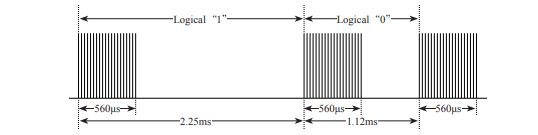
\includegraphics[width=\linewidth]{figure/4-2}
	\caption{NEC的0,1码}
	\label{fig:4-2}
\end{figure}

重复码的格式是由9ms的高电平和2.25ms 的低电平及一个560$\mu$s的高电平组成

发送格式如下:
NEC 协议中,首先是9ms的高电平脉冲,其后是 4.5ms 的低电平,接下来就是 8bit 的地址码(从低有效位开始发),而后是 8bit 的地址码的反码(主要是用于校验是否出错)。然后是 8bit 的命令码(也是从低有效位开始发),而后也是 8bit 的命令码的反码。
\begin{figure}[htbp]
	\centering
	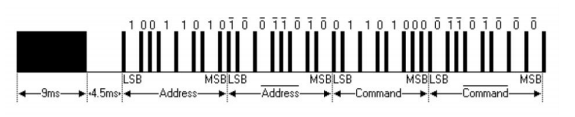
\includegraphics[width=\linewidth]{figure/4-3}
	\caption{NEC编码}
	\label{fig:4-3}
\end{figure}

2. RC5 协议
RC5 协议由 Philips 公司推出。它采用载波频率固定为36kHz 的 ASK 调制和曼彻斯特编码。
基本特征:
(1)4 位地址位,4 位命令位。
(2)地址位和命令位被传输一次。
(3)载波频率36kHz。
(4)每一位的时间为1.05ms 或 2.1ms。

逻辑 0 和 1 的定义如:
逻辑 1 的是由889$\mu$s 的低电平和889$\mu$s 的高电平组成的脉冲表示。
逻辑 0 的是由889$\mu$s 的高电平和889$\mu$s 的低电平组成的脉冲表示。
\begin{figure}[htbp]
	\centering
	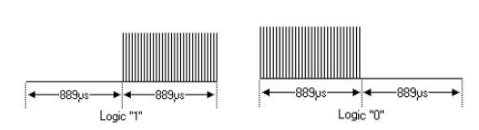
\includegraphics[width=\linewidth]{figure/4-4}
	\caption{RC5的0,1编码}
	\label{fig:4-4}
\end{figure}

发送格式如下:
RC5 协议中,首先是“110”的信号,接下来就是 5bit 的地址码。然后是 7bit 的命令码。
\begin{figure}[htbp]
	\centering
	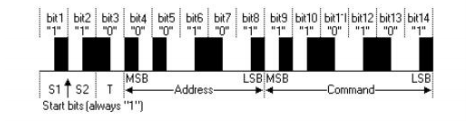
\includegraphics[width=\linewidth]{figure/4-5}
	\caption{RC5编码}
	\label{fig:4-5}
\end{figure}

为了提高红外编码的识别效率,需要引用一个IRremote库函数。在编写基于红线传感器收发通信的Arduino应用程序时,这个开源库函数可极大地减少我们的编码工作量和程序代码量。库函数硬件上支持多种Arduino主控板,软件上支持多种红外遥控编码的发送和接收协议,而且便于扩展和用户自定义。

本次系统开发过程中,针对通用空调红外遥控器,编写了以下Arduino的红外解码程序用于控制空调温度:
\begin{lstlisting}[language=C,title=代码4-1: Arduino的红外解码程序]
#include <Arduino.h>

/*
	* Define macros for input and output pin etc.
	*/
#include "PinDefinitionsAndMore.h"

/*
	* You can change this value accordingly to the receiver module you use.
	* The required value can be derived from the timings printed here.
	* Keep in mind that the timings may change with the distance
	* between sender and receiver as well as with the ambient light intensity.
	*/
#define MARK_EXCESS_MICROS    20 // recommended for the cheap VS1838 modules

//#define RECORD_GAP_MICROS 12000 // Activate it for some LG air conditioner protocols
#include <IRremote.h>

//+=============================================================================
// Configure the Arduino
//
void setup() {
	pinMode(LED_BUILTIN, OUTPUT);

	Serial.begin(9600);   // Status message will be sent to PC at 9600 baud
#if defined(__AVR_ATmega32U4__) || defined(SERIAL_USB) || defined(SERIAL_PORT_USBVIRTUAL)  || defined(ARDUINO_attiny3217)
	delay(4000); // To be able to connect Serial monitor after reset or power up and before first print out. Do not wait for an attached Serial Monitor!
#endif
	// Just to know which program is running on my Arduino
	Serial.println(F("START " __FILE__ " from " __DATE__ "\r\nUsing library version " VERSION_IRREMOTE));

	IrReceiver.begin(IR_RECEIVE_PIN, ENABLE_LED_FEEDBACK); // Start the receiver, enable feedback LED, take LED feedback pin from the internal boards definition

	Serial.print(F("Ready to receive IR signals at pin "));
	Serial.println(IR_RECEIVE_PIN);
}

//+=============================================================================
// The repeating section of the code
//
void loop() {
	if (IrReceiver.decode()) {  // Grab an IR code
		// Check if the buffer overflowed
		if (IrReceiver.decodedIRData.flags & IRDATA_FLAGS_WAS_OVERFLOW) {
			Serial.println("IR code too long. Edit IRremoteInt.h and increase RAW_BUFFER_LENGTH");
		} else {
			Serial.println();                               // 2 blank lines between entries
			Serial.println();
			IrReceiver.printIRResultShort(&Serial);
			Serial.println();
			Serial.println(F("Raw result in internal ticks (50 us) - with leading gap"));
			IrReceiver.printIRResultRawFormatted(&Serial, false); // Output the results in RAW format
			Serial.println(F("Raw result in microseconds - with leading gap"));
			IrReceiver.printIRResultRawFormatted(&Serial, true);  // Output the results in RAW format
			Serial.println();                               // blank line between entries
			Serial.print(F("Result as internal ticks (50 us) array - compensated with MARK_EXCESS_MICROS="));
			Serial.println(MARK_EXCESS_MICROS);
			IrReceiver.compensateAndPrintIRResultAsCArray(&Serial, false); // Output the results as uint8_t source code array of ticks
			Serial.print(F("Result as microseconds array - compensated with MARK_EXCESS_MICROS="));
			Serial.println(MARK_EXCESS_MICROS);
			IrReceiver.compensateAndPrintIRResultAsCArray(&Serial, true); // Output the results as uint16_t source code array of micros
			IrReceiver.printIRResultAsCVariables(&Serial);  // Output address and data as source code variables

			IrReceiver.compensateAndPrintIRResultAsPronto(&Serial);
//        }
		}
		IrReceiver.resume();                            // Prepare for the next value
	}
}
\end{lstlisting}

\subsection{对开源项目的有效利用}

开放源代码软件(OSS)是一种计算机软件,其源代码提供许可证,版权持有者有权为任何目的研究,更改和分发软件给任何人。开源软件可能会以公开的协作方式开发。根据研究它的科学家,开源软件是开放式协作的一个突出例子。

对于开发者而言,了解并使用目前在社区中比较流行的开源项目是很必要的一件事。利用这些项目,项目开发工作有时能达到事半功倍的效果。尤其是在互联网这个飞速发展的领域,快速开发、快速上线就是生命,引入开源项目可以节省很多的人力和时间,降低开发成本。Standish Group 2008年的一份报告指出,采用开源软件模式每年可为消费者节省约600亿美元(480亿英镑)的费用。但采用开源软件的决定不应仅仅以低成本为基础。在切换到开源以充分利用它之前,需要对需求进行详细的分析和理解。

包管理器是现在 web 开发必须使用的工具,因为网站系统的开发有必要借助数以万计的众多开源爱好者们的力量。本系统由以下包管理系统提供支持:Python的包安装程序 pip,Ubuntu Linux发行版的包管理器APT。pip是Python官方推荐的包管理工具:属于python的一部分。pip 也支持直接从文件读取包列表以便批量安装,通常命名为 requirements.txt。下面列出了本系统全部所用的python模块。通过requirements.txt可以方便有效的做出系统的迁移部署。APT可以方便快捷的部署各种类型服务,如本系统中采用的MQTT服务器,WEB服务器等。都可以直接通过\begin{lstlisting}[language=bash]
apt install mosquitto nginx
\end{lstlisting}一句命令直接安装,免去了windows系统下,寻找,下载,安装的方式,节省了大量的时间。

\begin{lstlisting}[title=温控系统所选用的全部Python模块以及版本列表]
alembic==1.0.10
aniso8601==7.0.0
Click==7.0
Flask==1.0.3
Flask-Admin==1.5.3
Flask-Login==0.4.1
Flask-Migrate==2.5.2
Flask-MQTT==1.0.5
Flask-RESTful==0.3.7
Flask-Restless==0.17.0
Flask-SocketIO==4.2.0
Flask-SQLAlchemy==2.4.0
Flask-WTF==0.14.2
itsdangerous==1.1.0
Jinja2==2.10.1
Mako==1.0.12
MarkupSafe==1.1.1
mimerender==0.6.0
paho-mqtt==1.4.0
python-dateutil==2.8.0
dj-database-url==0.5.0
python-editor==1.0.4
python-engineio==3.9.0
python-mimeparse==1.6.0
python-socketio==4.3.0
pytz==2019.2
six==1.12.0
SQLAlchemy==1.3.4
typing==3.7.4
Werkzeug==0.15.4
WTForms==2.2.1
gunicorn==20.1.0 
mysqlclient==1.4.2.post1
requests==2.22.0
\end{lstlisting}

上表列出了温控系统所选用的全部Python模块以及版本列表,可以看到数目相当多,而正是利用了这些方便的开源项目,才使得快速开发一个稳定、强大的温控系统成为可能。

需要注意的是,开源许可软件大多免费提供,但这不一定是这种情况。某些仅允许非商业性质的再分发,或修改源代码仅供个人使用的软件并不属于开源。开放源代码可能有一些限制,特别是关于表达对软件起源的限制,例如要求在代码中保留作者姓名和版权声明,或者要求重新分发许可软件仅在相同的许可证下发布。

本次系统的开发遵循了开源许可协议,其诞生离不开众多开源项目的支持,在此对这些开源项目作者所做出的工作表示感谢。
